\subsection{Teorema Pythaogras}
Salah satu teorema paling terkenal di kalangan awam (atau setidaknya di pop culture). Diberikan segitiga $ABC$ dengan sudut $C$ siku-siku. Jika panjang sisi $AB=c$, $BC=a$, dan $CA=b$, maka berlaku
\begin{align*}
    a^2+b^2=c^2
\end{align*}
\begin{center}
    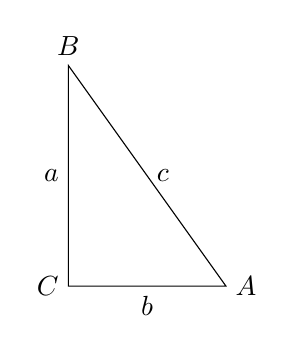
\begin{tikzpicture}
    % titik-titik segitiga
    \coordinate[label=left:$C$]  (C) at (-1.5cm,-1.cm);
    \coordinate[label=above:$B$] (B) at (-1.5cm,1.8cm);
    \coordinate[label=right:$A$] (A) at (0.5cm,-1.cm);
    
    % pembuatan segitiga
    \draw (A) -- node[right]{$c$} (B)  -- node[left]{$a$} (C) -- node[below]{$b$} cycle;
    \end{tikzpicture}
\end{center}
\subsection{Latihan Soal Pythagoras}
\begin{enumerate}
    \item (OSK SMP 2016) Diketahui $ABCD$ dan $CEGH$ adalah dua persegipanjang kongruen dengan panjang $17$ cm, dan lebar $8$ cm. Titik $E$ berada di sisi $AB$ dan $D$ berada di sisi $GH$. Titik $F$ adalah titik potong sisi $AD$ dan $EG$. Luas segiempat $EFDC$ adalah .... $cm^2$.

    \item Misalkan $ABC$ adalah segitiga lancip. Titik $D$, $E$, dan $F$ terletak pada sisi $BC$, $CA$, dan $AB$, berturut-turut, sedemikian sehingga $AD$, $BE$, dan $CF$ adalah garis tinggi segitiga $ABC$. Titik $H$ adalah titik tinggi segitiga $ABC$. Jika $DE = 8$, $DF = 15$, dan $EF = 17$, tentukan panjang $AH$.
\end{enumerate}